\let\negmedspace\undefined
\let\negthickspace\undefined
\documentclass[journal]{IEEEtran}
\usepackage[a5paper, margin=10mm, onecolumn]{geometry}
%\usepackage{lmodern} % Ensure lmodern is loaded for pdflatex
\usepackage{tfrupee} % Include tfrupee package

\setlength{\headheight}{1cm} % Set the height of the header box
\setlength{\headsep}{0mm}     % Set the distance between the header box and the top of the text

\usepackage{gvv-book}
\usepackage{gvv}
\usepackage{cite}
\usepackage{amsmath,amssymb,amsfonts,amsthm}
\usepackage{algorithmic}
\usepackage{graphicx}
\usepackage{textcomp}
\usepackage{xcolor}
\usepackage{txfonts}
\usepackage{listings}
\usepackage{enumitem}
\usepackage{mathtools}
\usepackage{gensymb}
\usepackage{comment}
\usepackage[breaklinks=true]{hyperref}
\usepackage{tkz-euclide} 
\usepackage{listings}
% \usepackage{gvv}                                        
\def\inputGnumericTable{}                                 
\usepackage[latin1]{inputenc}                                
\usepackage{color}                                            
\usepackage{array}                                            
\usepackage{longtable}                                       
\usepackage{calc}                                             
\usepackage{multirow}                                         
\usepackage{hhline}                                           
\usepackage{ifthen}                                           
\usepackage{lscape}
\begin{document}

\bibliographystyle{IEEEtran}
\vspace{3cm}

\title{1.1.6.27}
\author{EE24BTECH11057 - SHIVAM SHILVANT*}
% \maketitle
% \newpage
% \bigskip
{\let\newpage\relax\maketitle}

\renewcommand{\thefigure}{\theenumi}
\renewcommand{\thetable}{\theenumi}
\setlength{\intextsep}{10pt} % Space between text and floats


\numberwithin{equation}{enumi}
\numberwithin{figure}{enumi}
\renewcommand{\thetable}{\theenumi}


\textbf{Question}:\\
Prove that the three points  $\brak{-4,6,10}$, $\brak{2,4,6}$ and $\brak{14,0,-2}$ are collinear.\\
If the points are collinear , then their determinant should equal to 0.
\begin{align}
 \mydet {-4 & 6 & 10 \\ 2 & 4 & 6 \\ 14 & 0 & -2} = 0 \label{1.6.9.1}
\end{align}
expanding the det by column 3.
\begin{align}
 \brak{-2}\mydet {-4 & 6 \\ 2 & 4} - 6\mydet{ -4 & 6 \\14 & 0 } + 10\mydet { 2 & 4 \\ 14 & 0 } &= 0& \\
 \brak{-2}\brak{-28} - \brak{6}\brak{-84} + \brak{10}\brak{-56} &= 0& \\
 56 + 504 - 560 &= 0& \\
 0 &= 0& \\
\end{align}
So, as the determinant is zero , All the three points are collinear.
\begin{figure}[h!]
   \centering
   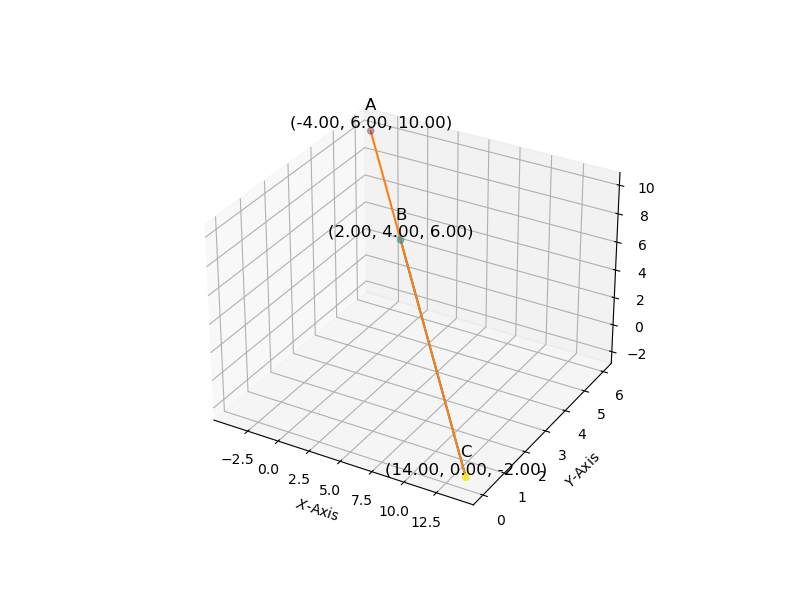
\includegraphics[width=0.7\linewidth]{figs/Figure_1.png}
   \caption{Stem Plot of y\brak{n}}
   \label{stemplot}
\end{figure}
\end{document}  
\end{document}

